The last few chapters introduced some of the most widely used algorithms based on Bayes' filter for probabilistic robot localization and state estimation. However these fundamental algorithms still need further enhancements before application to many robot localization tasks, since in their standard form they don't incorporate a notion of a local \textit{map}. For example, a particle filter could be applied in its original form to a problem of global localization based on GNSS measurements, but localizing based on range measurements requires knowledge about \textit{what} object is being ranged, and \textit{where} that object is with respect to the local environment (i.e. the map).
In this chapter a more specific definition of mobile robot localization is considered\cite{ThrunBurgardEtAl2005}, namely the problem of determining the pose of a robot relative to a \textit{given map} of the environment.

\notessection{Robot Localization}
Localization with respect to a map can be interpreted as a problem of coordinate transformation. Maps are described in a global coordinate system, which is independent of a robot’s pose. Localization can then be viewed as the process of establishing a correspondence between the map coordinate system and the robot’s local coordinate system. Knowing this coordinate transformation then enables the robot to express the location of objects of interest within its own coordinate frame (a necessary prerequisite for robot autonomy).


In 2D problems, knowing the pose $\x_t = [x, y, \theta]^\top $ of a robot is sufficient to establish this correspondence, and an ideal sensor would directly be able to measure this pose. However in practice no such sensor exists, and therefore \textit{indirect} (often noisy) measurements $\z_t$ of the pose are used. Since it is almost impossible to be able to reliably estimate $\x_t$ from a single measurement $\z_t$, localization algorithms typically integrate additional data \textit{over time} to build reliable localization estimates. For example, consider a robot located inside a building where many corridors look alike. In this case a single sensor measurement (e.g. a range scan) is usually insufficient to disambiguate the identity of the corridor from the others.

In this chapter it will be seen how this map-based localization problem can be cast in the Bayesian filtering framework, such that the algorithms from previous chapters can be leveraged.


\subsection{A Taxonomy of Localization Problems}
To understand the broad scope of challenges related to robot localization, it is useful to develop a brief taxonomy of localization problems. This categorization will divide localization problems along a number of important dimensions pertaining to the nature of the environment (e.g. static versus dynamic), the initial knowledge that a robot may possess, and how information about the environment is gathered (e.g. passive or active, with one robot or collaboratively with several robots).

\subsubsection{Local vs. Global}
Localization problems can be characterized by the type of knowledge that is available initially, which has a significant impact on what type of localization algorithm is most appropriate for the problem.

\begin{itemize}
    \item \textit{Position tracking} problems assume that the initial pose of the robot is known. In these types of problems only incremental updates are required (i.e. the localization error is generally always small), and therefore unimodal Gaussian filters (e.g. Kalman filters) can be efficiently applied.
    
    \item \textit{Global localization} problems assume that the initial pose of the robot is unknown. In these scenarios the use of a unimodal parametric belief distribution cannot adequately capture the global uncertainty. Therefore it is more appropriate to use non-parametric, multi-hypothesis filters, such as the particle filter.
    
    \item The \textit{kidnapped robot problem} is a variant of the global localization problem (i.e. unknown initial pose) where the robot can get ``kidnapped'' and ``teleported'' to some other location. This problem is more difficult than the global localization problem since the localization algorithm needs to have an awareness that sudden drastic to the robot's pose are possible. While robots are typically not ``kidnapped'' in practice, the consideration of this type of problem is useful for ensuring the localization algorithm is \textit{robust}, since the ability to recover from failure is essential for truly autonomous robots. Similar to the global localization problem, these problems are often best addressed using non-parametric, multi-hypothesis filters.
\end{itemize}

\subsubsection{Static vs. Dynamic}
Environmental changes are another important consideration in mobile robot localization, specifically whether they are static or dynamic.
\begin{itemize}
    \item In \textit{static} environments the robot is the only object that moves. Static environments are generally much easier to perform localization in.
    \item \textit{Dynamic} environments possess objects other than the robot whose locations or configurations change over time. This problem is usually addressed by augmenting the state vector to include the movement of dynamic entities, or by filtering the sensor data to remove the effects of environment dynamics.
\end{itemize}

\subsubsection{Passive vs. Active}
Information collected via measurements is crucial for robot localization. Therefore it is reasonable to consider localization problems where the robot can \textit{explicitly} choose its actions to gather more (or more specific) information from the environment. 
\begin{itemize}
    \item \textit{Passive localization} problems assume that the robot's motion is unrelated to its localization process.
    \item \textit{Active localization} problems consider the ability of the robot to choose its actions (at least partially) to improve its understanding of the environment. For example, a robot in the corner of a room might choose to reorient itself to face the rest of the room, so it can collect environmental information as it moves along the wall. Hybrid approaches are also possible, since it may be inefficient to use active localization all of the time. 
\end{itemize}

\subsubsection{Single Robot vs. Multi-Robot}
It is of course also possible to consider problems where several robots all gather independent information and then share that information with each other.
\begin{itemize}
    \item \textit{Single-robot localization} problems are the most commonly studied and utilized approach, and are often simpler because all data is collected on a single platform.
    \item \textit{Multi-robot localization} problems consider teams of robots that share information in such a way that one robot's belief can be used to influence another robot's belief if the relative location between robots is known. 
\end{itemize}


\subsection{Robot Localization via Bayesian Filtering}
The parametric (e.g. EKF) and non-parametric (e.g. particle) filters from the previous chapters are all variations of the Bayes filter. In particular they rely on a Markov process assumption and the identification of probabilistic measurement models. In this section it is shown how map-based robot localization can be cast into this framework, such that the previously discussed algorithms can be applied.

Similar to the general filtering context from the previous chapters, at time $t$ the state is denoted by $\x_t$, the control input is denoted by $\bu_t$, and the measurements are denoted by $\z_t$. For example, a differential drive robot equipped with a laser range-finder (returning a set of range measurements $r_i$ and bearings $\phi_i$), the state, control, and measurements would be:
\begin{equation}
\x_{t} = \begin{bmatrix} x \\ y \\ \theta
\end{bmatrix}, \quad
\bu_{t} = \begin{bmatrix} v \\ \omega 
\end{bmatrix}, \quad
\z_{t} =  \begin{bmatrix} r_1 \\ \phi_1 \\  \vdots
\end{bmatrix}.
\end{equation}

However, the critical new component is the concept of a \textit{map} (denoted as $\m$), which is a list of objects in the environment along with their properties:
\begin{equation}
\m = \{ m_1 , m_2 , \ldots , m_N \},
\end{equation}
where $m_i$ represents the properties of a specific object. Generally there are two types of maps that will be considered, location-based maps and feature-based maps, which typically have differences in both computational efficiency and expressiveness.

For location-based maps, the index $i$ associated with object $m_i$ corresponds to a specific \textit{location} (i.e. $m_i$ are volumetric objects). For example, objects $m_i$ in a location-based map might represent cells in a cell decomposition or grid representation of a map (see Figure \ref{fig:LocationBasedMaps}).
\begin{figure}[ht]
\centering
\includegraphics[width=.75\linewidth]{tex/figs/ch16_figs/location_based_maps.png}
\caption{Two examples of location-based maps, both represent the map as a set of volumetric objects (i.e. cells in these cases).}
\label{fig:LocationBasedMaps}
\end{figure}
One potential disadvantage of the cell-based maps is that their resolution is dependent on the size of the cells, but their advantage is that they can explicitly encode information about presence (or absence) of objects in specific locations.

% The first example of a location-based map employs vertical cell decomposition. This method essentially sweeps a vertical line through the width of the environment, and every time a corner is encountered, a cell is built. The result is a set of trapezoidal cells as shown in Fig. \ref{fig:LocationBasedMaps}, left. Each element of the map vector would be one of the cells. It is important to note that this technique can only describe the location of the robot using the presence or absence of the robot in a cell, but cannot give information on where within a cell the robot may be. The second common example of a location-based map uses fixed cell decomposition (Fig. \ref{fig:LocationBasedMaps}, right). In this grid map, the $i$th element of the map corresponds to the vector $x_i$ position of the $i$-th cell of the grid map. Thus, each cell represents a map vector. As compared the the fixed cell decomposition, the vertical cell decomposition is more efficient, as it abstracts the environment as a graph with nodes and edges. However, fixed cell decomposition can have better spatial resolution at the expense of additional computational complexity. Both techniques can give both the presence and absence of an object, which cannot be done with feature-based maps.

For feature-based maps, an index $i$ is a feature index, and $m_i$ contains information about the properties of that feature, including its Cartesian location. These types of maps can typically be thought of as a collection of landmarks. Figure \ref{fig:FeatureBasedMaps} gives two examples of feature-based maps, one which is represented by a set of lines, and another which is represented by nodes and edges like a graph (i.e. a topological map).
\begin{figure*}[ht]
\centering
\includegraphics[width=0.8\linewidth]{tex/figs/ch16_figs/feature_based_maps.png}
\caption{Two examples of feature-based maps.}
\label{fig:FeatureBasedMaps}
\end{figure*}
Feature-based maps can be more finely tuned to specific environments, for example the line-based map might make sense to use in highly structured environments such as buildings. While feature-based maps can be computationally efficient, their main disadvantage is that they typically do not capture spatial information about all potential obstacles.

\subsubsection{State Transition Model}
In the previous chapters on Bayesian filtering the probabilistic state transition model $p(\x_t \mid \bu_t, \x_{t-1})$ describes the posterior distribution over the states that the robot could transition to when executing control $\bu_t$ from $\x_{t-1}$. However in robot localization problems it might be important to take into account how the map $\m$ could affect the state transition since in general:
\begin{equation*}
p(\x_t \mid \bu_t, \x_{t-1}) \neq p(\x_t \mid \bu_t, \x_{t-1}, \m).
\end{equation*}
For example, $p(\x_t \mid \bu_t, \x_{t-1})$ cannot account for the fact that a robot cannot move through walls since it doesn't know that walls exist!

However, a common approximation is to make the assumption that:
\begin{equation} \label{eq:statetransmap}
p(\x_t \mid \bu_t, \x_{t-1}, \m) \approx \eta \frac{p(\x_{t}\mid \bu_{t}, \x_{t-1} ) p(\x_{t} \mid \m )}{p(\x_{t})},
\end{equation}
where $\eta$ is a normalization constant. This approximation can be derived from Bayes' rule by assuming that $p(\m \mid \x_t, \x_{t-1}, \bu_t) \approx p(\m \mid \x_t)$ (which is a tight approximation under high update rates). More specifically:
\begin{equation*}
\begin{split}
p(\x_t \mid \bu_t, \x_{t-1}, \m) &= \frac{p(\m | \x_{t}, \x_{t-1}, \bu_{t}) p(\x_{t} \mid \x_{t-1}, \bu_t)}{p(\m \mid \x_{t-1}, \bu_{t})}, \\
&= \eta' p(\m | \x_{t}, \x_{t-1}, \bu_{t}) p(\x_{t} \mid \x_{t-1}, \bu_t), \\
&\approx \eta' p(\m | \x_{t}) p(\x_{t} \mid \x_{t-1}, \bu_t), \\
& =\eta \frac{p(\x_{t}\mid \bu_{t}, \x_{t-1} ) p(\x_{t} \mid \m )}{p(\x_{t})},
\end{split}
\end{equation*}
where $\eta'$ and $\eta$ are normalization constants (such that the total probability density integrates to one).

In this approximation the term $p(\x_{t} \mid \m )$ is the state probability conditioned on the map which can be thought of as describing the ``consistency'' of state with respect to the map. The approximation \eqref{eq:statetransmap} can therefore be viewed as making a probabilistic guess using the original state transition model (without map knowledge), and then using the consistency term $p(\x_{t} \mid \m )$ to check the plausibility of the new state $\x_t$ given the map.

% \begin{figure}[ht]
% \centering
% \includegraphics[width=.5\linewidth]{tex/figs/ch16_figs/ProbabilisticMotion.png}
% \caption{Probabilistic Motion}
% \label{fig:ProbabilisticMotion}
% \end{figure}

\subsubsection{Measurement Model}
The probabilistic measurement model model $p(\z_t \mid \x_t)$ from previous chapters also needs to be modified to take map information into account. This new measurement model can simply be expressed as $p(\z_t \mid \x_t, \m)$ (i.e. measurement is also conditioned on the map). This is obviously important because the local measurements can have significant influence from the environment. For example a range measurement is dependent on what object is currently in the line of sight.

Additionally, since the suite of sensors on a robot may generate more than one measurement when queried, it is also common to make another measurement model assumption for simplicity. Suppose $K$ measurements are taken at time $t$, such that:
\begin{equation*}
    \z_t = \begin{bmatrix}
    \z_t^1 \\ \vdots \\ \z_t^K
    \end{bmatrix}.
\end{equation*}
Then it can often be assumed that each of the $K$ measurements are conditionally independent from each other (i.e. when conditioned on $\x_t$ and $\m$ the probability of measuring $\z_t^k$ is independent from the other measurements). With this assumption the probabilistic measurement model can be expressed as:
\begin{equation} \label{eq:condind}
    p(\z_{t} \mid \x_{t}, \m) = \prod_{k=1}^{K}p(\z_{t}^{k}\mid \x_{t}, \m).
\end{equation}

\subsection{Markov Localization}
With the probabilistic state transition and measurement models that include the map, the Bayes' filter can be directly modified as shown in Algorithm \ref{alg:markovloc}.
\begin{algorithm}[ht]
 \KwData{$bel(\x_{t-1}), \bu_{t},\z_{t}, \m$}
 \KwResult{$bel(\x_{t})$}
 \ForEach{$\x_t$}{
    $\overline{bel}(\x_t) = \int p(\x_t\mid \bu_{t}, \x_{t-1},\m) bel(\x_{t-1}) d\x_{t-1}$ \\
    $bel(\x_t) = \eta p(\z_t\mid \x_{t},\m)\overline{bel}(\x_t)$
 }
 \Return $bel(\x_{t})$
 \caption{Markov Localization Algorithm}
 \label{alg:markovloc}
\end{algorithm}
As can be seen, this algorithm is conceptually identical to the Bayes' filter except for the inclusion of the model $\m$. This algorithm is referred to as the \textit{Markov localization} algorithm, and the localization problem it is trying to solve is generally referred to as simply \textit{Markov localization}\footnote{Recall the use of the Markov property assumption in the derivation of the Bayes' filter.}. 

The Markov localization algorithm can be used to address global localization, position tracking, and kidnapped robot problems, but generally some implementation details might be different. The choice for the initial (prior) belief distribution $bel(\x_0)$ is one such parameter that may be different depending on the type of localization problem.

Specifically, since the initial belief encodes any prior knowledge about the robot pose, the best choice of distribution depends on what (if any) knowledge is available. For example, in the position tracking problem it is assumed that an initial pose of the robot is known. Therefore choosing a (unimodal) Gaussian distribution $bel(\x_0) \sim \mathcal{N}(\bar{\x}_0, \bSigma_0)$ with a small covariance might be a good choice. Alternatively, for a global localization problem the initial pose is not known. In this case an appropriate choice for the initial belief would be a uniform distribution $bel(\x_0) = 1/\lvert X \rvert$ over all possible states $\x$.

Similarly to the original Bayes' filter from previous chapters, the Markov localization algorithm \ref{alg:markovloc} is generally not possible to implement in a computationally tractable way. However, practical implementations can still be developed by again leveraging some sort of structure to the belief distribution $bel(\x_t)$ (e.g. through Gaussian or particle representations). Two commonly used implementations based on specific structured beliefs will now be discussed: extended Kalman filter localization and Monte Carlo localization.

% \begin{figure}[ht]
% \centering
% \includegraphics[width=.8\linewidth]{tex/figs/ch16_figs/MarkovLocalizationPic.png}
% \caption{Markov Localization Illustration. We consider a robot moving along a wall with three doors (a) The belief is initialized with a uniform distribution. (b) The robot moves to the first door and makes an observation. We apply the correction step to update our belief (c) The robot moves to the second door. The shifted belief is flattened because there is uncertainty with how much we moved. (d) We take a second observation, apply the correction, and obtain a large peak in the posterior belief. (e) The robot’s belief after moving further down the wall}
% \label{fig:MarkovLocalizationPic}
% \end{figure}

\subsection{Extended Kalman Filter (EKF) Localization}
The extended Kalman filter (EKF) localization algorithm is essentially equivalent to the EKF algorithm presented in previous chapters, except that it also takes the map $\m$ into account. In particular, it still makes a Guassian belief assumption, $bel(\x_t) \sim \mathcal{N}(\bmu_t, \bSigma_t)$, to add structure to the filtering problem. As a brief review, the assumed state transition model is given by:
\begin{equation*}
\x_t = g(\bu_t, \x_{t-1}) + \bm{\epsilon}_t,
\end{equation*}
where $\bm{\epsilon}_t \sim \mathcal{N}(\bm{0}, \bm{R}_t)$ is Gaussian zero-mean noise. The Jacobian $G_t$ is again defined by $G_t = \nabla_{\x}g(\bu_t, \bmu_{t-1})$, where $\bmu_{t-1}$ is the expected value of the previous belief distribution $bel(\x_{t-1})$. 

The main difference in EKF localization is the assumption that a feature-based map is available, consisting of point landmarks given by:
\begin{equation*}
\m = \{m_1, m_2, \dots, m_N\}, \quad m_j = (m_{j,x}, m_{j,y}),
\end{equation*}
where $N$ is the total number of landmarks, and each landmark $m_j$ encapsulates the location $(m_{j,x}, m_{j,y})$ of the landmark in the global coordinate frame. Measurements $\z_t$ associated with these point landmarks at a time $t$ are denoted by:
\begin{equation*}
\z_t = \{\z_t^1, \z_t^2, \dots \},
\end{equation*}
where $\z_t^i$ is associated with a particular landmark and is assumed to be generated by the measurement model:
\begin{equation*}
\z^i_t = h(\x_t, j, \m) + \bm{\delta}_t,
\end{equation*}
where $\bm{\delta}_t \sim \mathcal{N}(\bm{0}, \bm{Q}_t)$ is Gaussian zero-mean noise and $j$ is the index of the map feature $m_j \in \m$ that measurement $i$ is associated with.

One fundamental problem that now needs to be addressed is the \textit{data association problem}, which arises due to uncertainty in which measurements are associated with which landmark. To begin addressing this problem, the correspondences are modeled through a variable $c_t^i \in \{1,\dots,N+1\}$, which take on the values $c_t^i = j$ if measurement $i$ corresponds to landmark $j$, and $c_t^i = N + 1$ if measurement $i$ has no corresponding landmark. 
Then, given a correspondence $c^i_t$ of measurement $i$ (associated with a specific landmark), the Jacobian $H^i_t$ used in the EKF measurement correction step can be determined. Specifically, for the $i$-th measurement the Jacobian of the new measurement model can be computed by $H^{c^i_t}_t = \nabla_{\x}h(\bar{\bmu}_t,c^i_t,\m)$, where $\bar{\bmu}_t$ is the predicted mean (that results from the EKF prediction step).


\subsubsection{EKF Localization with Known Correspondences}
In practice the correspondences between measurements $\z^i_t$ and landmarks $m_j$ are generally unknown. However, it is useful from a pedagogical standpoint to first consider the case where these correspondences $\bc_t = [c_t^1,\dots]^\top $ are assumed to be \textit{known}.

In the EKF localization algorithm given in Algorithm \ref{alg:ekflocal}, the main difference from the original EKF filter algorithm is that multiple measurements are processed at the same time. Crucially, this is accomplished in a computationally efficient way by exploiting the conditional independence assumption \eqref{eq:condind} for the measurements. In fact, by exploiting this assumption and some special properties of Gaussians, the multi-measurement update can be implemented by just looping over each measurement individually and applying the standard EKF correction.
\begin{algorithm}[ht]
 \KwData{$\bmu_{t-1}, \bSigma_{t-1}, \bu_{t},\z_{t}, \bc_t, \m$}
 \KwResult{$\bmu_t, \bSigma_t$}
 $\bar{\bmu}_t = g(\bu_t,\bmu_{t-1})$\\
 $\bar{\bSigma}_t = G_t\bSigma_{t-1} G_t^{T} + \bm{R}_t$\\
 \ForEach{$\z_t^i$}{
  $j = c_t^i$\\
  $S_t^i = H_t^j\bar{\bSigma}_{t}[H^j_t]^{T}+\bm{Q}_t$\\
  $K^i_t = \bar{\bSigma}_{t}[H^j_t]^{T}[S_t^i]^{-1}$\\
  $\bar{\bmu}_t = \bar{\bmu}_t + K^i_t(\z^i_t - h(\bar{\bmu}_{t}, j, \m))$\\
  $\bar{\bSigma}_t = (I - K^i_t H^j_t)\bar{\bSigma}_t$\\
 }
 $\bmu_t = \bar{\bmu}_t$\\
 $\bSigma_t = \bar{\bSigma}_t$\\
 \Return $\bmu_t, \bSigma_t$
 \caption{Extended Kalman Filter Localization Algorithm}
 \label{alg:ekflocal}
\end{algorithm}

\subsubsection{EKF Localization with Unknown Correspondences}
For EKF localization with \textit{unknown} correspondences, the correspondence variables must also be estimated!
The simplest way to determine the correspondences online is to use maximum likelihood estimation, in which the most likely value of the correspondences $\bc_t$ is determined by maximizing the data likelihood:
\begin{equation*}
    \hat{\bc}_{t} = \arg \max_{\bc_{t}}p(\z_{t}\mid \bc_{1:t},\m,\z_{1:t-1},\bu_{1:t})
\end{equation*}
In other words, the set of correspondence variables is chosen to maximize the probability of getting the current measurement given the history of correspondence variables, the map, the history of measurements, and the history of controls. By marginalizing over the current pose $\x_t$ this distribution can be written as:
\begin{equation*}
\begin{split}
p(\z_{t}\mid \bc_{1:t},\m,\z_{1:t-1},\bu_{1:t}) &= \int p(\z_{t}\mid \bc_{1:t},\x_t, \m,\z_{1:t-1},\bu_{1:t}) p(\x_{t}\mid \bc_{1:t},\m,\z_{1:t-1},\bu_{1:t}) d\x_t, \\
&= \int p(\z_{t}\mid \bc_{t},\x_t, \m) \overline{bel}(\x_t) d\x_t. \\
\end{split}
\end{equation*}
Note that the term $p(\z_{t}\mid \bc_{1:t},\x_t, \m)$ is essentially the assumed measurement model given \textit{known} correspondences. Then, by again leveraging the conditional independence assumption for the measurements $\z_t^i$ from \eqref{eq:condind}, this can be written as:
\begin{equation*}
\begin{split}
p(\z_{t}\mid \bc_{1:t},\m,\z_{1:t-1},\bu_{1:t}) = \int \prod_i p(\z^i_{t}\mid c^i_{t},\x_t, \m) \overline{bel}(\x_t) d\x_t. \\
\end{split}
\end{equation*}
Importantly, each decision variable $c_t^i$ in the maximization of this quantity shows up in separate terms of the product! Therefore it is possible to maximize each parameter independently by solving the optimization problems:
\begin{equation*}
\begin{split}
\hat{c}^i_{t} = \arg \max_{c^i_{t}} \int p(\z^i_{t}\mid c^i_{t},\x_t, \m) \overline{bel}(\x_t) d\x_t. \\
\end{split}
\end{equation*}
This problem can be solved quite efficiently since it is assumed that the measurement models and belief distributions are Gaussian\footnote{Similar to the previous chapters, in this case the product of terms inside the integral will be Gaussian since both terms are Gaussian.}. In particular, the probability distribution resulting from the integral is a Gaussian with mean and covariance:
\begin{equation*}
\begin{split}
\int p(\z^i_{t}\mid c^i_{t},\x_t, \m) \overline{bel}(\x_t) d\x_t \sim \mathcal{N}(h(\bar{\bmu}_t, c_t^{i}, \m), H_t^{c_t^i} \bar{\bSigma}_t [H_t^{c_t^i}]^\top  + \bm{Q}_t).
\end{split}
\end{equation*}
The maximum likelihood optimization problem can therefore be expressed as:
\begin{equation*}
\begin{split}
\hat{c}^i_{t} = \arg \max_{c^i_{t}} \:\:\mathcal{N}(\z_t^i \mid \hat{\z}^{c_t^i}_t,\: S_t^{c_t^i}), \\
\end{split}
\end{equation*}
where $\hat{\z}^{j}_t = h(\bar{\bmu}_t, j, \m)$ and $S_t^j = H_t^{j} \bar{\bSigma}_t [H_t^{j}]^\top  + \bm{Q}_t$.
To solve this maximization problem, recall the definition of the Gaussian distribution:
\begin{equation*}
\mathcal{N}(\z_t^i \mid \hat{\z}^{j}_t,\: S_t^{j}) = \eta\: \text{exp}\big( -\frac{1}{2}(\z_t^i-\hat{\z}^{j}_t)^\top  [S_t^{j}]^{-1} (\z_t^i-\hat{\z}^{j}_t) \big),
\end{equation*}
where $\eta$ is a normalization constant. Since the exponential function is monotonically increasing and since $\eta$ is a positive constant, the maximum likelihood estimation problem can be equivalently expressed as:
\begin{equation}
\begin{split}
\hat{c}^i_{t} = \arg \min_{c^i_{t}} \:\: d_t^{i,c^i_{t}}, \\
\end{split}
\end{equation}
where 
\begin{equation} \label{eq:mahalanobis}
d_t^{ij} = (\z_t^i-\hat{\z}^{j}_t)^\top  [S_t^{j}]^{-1} (\z_t^i-\hat{\z}^{j}_t),
\end{equation}
is referred to as the \textit{Mahalanobis distance}.

The EKF localization algorithm with unknown correspondences is very similar to Algorithm \ref{alg:ekflocal}, except with the addition of this maximum likelihood estimation step. This new algorithm is given in Algorithm \ref{alg:ekflocalunknowncorr}.
\begin{algorithm}[ht]
 \KwData{$\bmu_{t-1}, \bSigma_{t-1}, \bu_{t},\z_{t}, \m$}
 \KwResult{$\bmu_t, \bSigma_t$}
 $\bar{\bmu}_t = g(\bu_t,\bmu_{t-1})$\\
 $\bar{\bSigma}_t = G_t\bSigma_{t-1} G_t^{T} + \bm{R}_t$\\
 \ForEach{$\z_t^i$}{
    \ForEach{landmark $k$ in the map}{
      $\hat{\z}_t^k = h(\bar{\bmu}_{t}, k, \m)$\\
      $S_t^k = H_t^k\bar{\bSigma}_{t}[H^k_t]^{T}+\bm{Q}_t$\\
     }
  $j = \arg\min_k \:\: (\z_t^i-\hat{\z}^{k}_t)^\top  [S_t^{k}]^{-1} (\z_t^i-\hat{\z}^{k}_t)$\\
  $K^i_t = \bar{\bSigma}_{t}[H^j_t]^{T}[S_t^j]^{-1}$\\
  $\bar{\bmu}_t = \bar{\bmu}_t + K^i_t(\z^i_t - \hat{\z}_t^j)$\\
  $\bar{\bSigma}_t = (I - K^i_t H^j_t)\bar{\bSigma}_t$\\
 }
 $\bmu_t = \bar{\bmu}_t$\\
 $\bSigma_t = \bar{\bSigma}_t$\\
 \Return $\bmu_t, \bSigma_t$
 \caption{EKF Localization Algorithm, Unknown Correspondences}
 \label{alg:ekflocalunknowncorr}
\end{algorithm}


One of the disadvantages of using the maximum likelihood estimation is that it can be brittle with respect to outliers and in cases where there are equally likely hypothesis for the correspondence.
An alternative approach to estimating correspondences that is more robust to outliers is to use a \textit{validation gate}. In this approach the Mahalanobis smallest distance $d_t^{ij}$ must also pass a \textit{thresholding} test:
\begin{equation*}
(\z_t^i-\hat{\z}^{j}_t)^\top  [S_t^{j}]^{-1} (\z_t^i-\hat{\z}^{j}_t) \leq \gamma,
\end{equation*}
in order for a correspondence to be created.



\begin{example}[Differential Drive Robot with Range and Bearing Measurements] \label{ex:rangeandbearing}
\theoremstyle{definition}
Consider a differential drive robot with state $\x = [x, y, \theta]^\top $, and suppose a sensor is available on the robot which measures the range $r$ and bearing $\phi$ of landmarks $m_j \in \m$ relative to the robot’s local coordinate frame. Additionally, multiple measurements corresponding to different features can be collected at each time step:
\begin{equation*}
\z_t = \{[r_t^1,\phi_t^1]^\top , [r_t^2,\phi_t^2]^\top , \dots\},
\end{equation*}
where each measurement $\z_t^i$ contains the range $r_t^i$ and bearing $\phi_t^i$. 

Assuming the correspondences are known, the measurement model for the range and bearing is:
\begin{equation}
h(\x_t, j, \m)  = \begin{bmatrix}
\sqrt{(m_{j,x} - x)^{2} + (m_{j,y}- y)^{2}} \\
\text{atan2}(m_{j,y}- y, m_{j,x} - x) - \theta
\end{bmatrix}.
\end{equation}
The measurement Jacobian $H^j_t$ corresponding to a measurement from landmark $j$ is then given by:
\begin{equation}
H^j_t = \begin{bmatrix}
-\frac{m_{j,x} - \bar{\mu}_{t,x}}{\sqrt{(m_{j,x} - \bar{\mu}_{t,x})^2 + (m_{j,y} - \bar{\mu}_{t,y})^2}} & -\frac{m_{j,y} - \bar{\mu}_{t,y}}{\sqrt{(m_{j,x} - \bar{\mu}_{t,x})^2 + (m_{j,y} - \bar{\mu}_{t,y})^2}} & 0 \\
\frac{m_{j,y} - \bar{\mu}_{t,y}}{(m_{j,x} - \bar{\mu}_{t,x})^2 + (m_{j,y} - \bar{\mu}_{t,y})^2} & -\frac{m_{j,x} - \bar{\mu}_{t,x}}{(m_{j,x} - \bar{\mu}_{t,x})^2 + (m_{j,y} - \bar{\mu}_{t,y})^2} & -1
\end{bmatrix}.
\end{equation}
It is also common to assume that the covariance of the measurement noise is given by:
\begin{equation*}
\bm{Q}_t = \begin{bmatrix}
\sigma_r^2 & 0 \\ 0 & \sigma_\phi^2
\end{bmatrix},
\end{equation*}
where $\sigma_r$ is the standard deviation of the range measurement noise and $\sigma_\phi$ is the standard deviation of the bearing measurement noise. This diagonal covariance matrix is typically used since these two measurements can be assumed to be uncorrelated.
\end{example}


\subsection{Monte Carlo Localization (MCL)}
Another approach to Markov localization is the Monte Carlo localization (MCL) algorithm. This algorithm leverages the non-parametric particle filter algorithm from the previous chapter, and is therefore much better suited to solving \textit{global} localization problems (unlike EKF localization which only solves position tracking problems). MCL can also be used to solve the kidnapped robot problem through some small modifications, such as injecting new random particles at each step to ensure that a ``particle collapse'' problem does not occur.

As a brief review, the particle filter represents the belief $bel(\x_t)$ by a set of $M$ particles:
\begin{equation*}
\mathcal{X}_t \coloneqq \{\x_t^{[1]}, \x_t^{[2]},..., \x_t^{[M]}\},
\end{equation*}
where each particle $\x_t^{[m]}$ represents a hypothesis about the true state $\x_t$. At each step of the algorithm the state transition model is used to propagate forward the particles, and then the measurement model is used to resample particles based on the measurement likelihood. This algorithm is shown in Algorithm \ref{alg:montecarlo}, and is nearly identical to the particle filter algorithm except that the map $\m$ is used in the probabilistic state transition and measurement models.
\begin{algorithm}[ht]
 \KwData{$\mathcal{X}_{t-1}, \bu_{t}, \z_{t}, \m$}
 \KwResult{$\mathcal{X}_{t}$}
 $\bar{\mathcal{X}}_{t} = \mathcal{X}_t = \emptyset$\\
 \For{$m=1$ \KwTo $M$}{
  Sample $\bar{\x}_{t}^{[m]} \sim p(\x_t\mid \bu_t, \x_{t-1}^{[m]},\m)$\\
  $w_t^{[m]} = p(\z_t \mid \bar{\x}_{t}^{[m]},\m)$\\
  $\bar{\mathcal{X}}_{t} = \bar{\mathcal{X}}_{t} \cup \big(\bar{\x}_{t}^{[m]}, w_t^{[m]} \big)$\\
 }
 \For{$m=1$ \KwTo $M$}{
  Draw $i$ with probability $\propto w_t^{[i]}$\\
  Add $\bar{\x}_{t}^{[i]}$ to $\mathcal{X}_t$
 }
 \Return $\mathcal{X}_t$
 \caption{Monte Carlo Localization Algorithm}
 \label{alg:montecarlo}
\end{algorithm}